\documentclass[10pt]{beamer}

% Configuration {{{
\usepackage[utf8]{inputenc}
\usepackage[T2A]{fontenc} % T1 for English
\usepackage[english, russian]{babel}

\usepackage{mathtools}
\usepackage{graphicx}
\usepackage[multidot]{grffile}
\usepackage[labelsep=period]{caption}

\setbeamertemplate{caption}[numbered]
\setbeamertemplate{navigation symbols}{}
\usefonttheme[onlymath]{serif}
\usepackage{DejaVuSansCondensed} % helvet for English
\usetheme{Madrid}

\linespread{1.2}
% }}}

\title[Взрывы сверхновых]{Взрывы сверхновых}
\author[Керим Гусейнов]{Керим Гусейнов}
\institute[]{Московский государственный университет имени М.\,В.~Ломоносова \\ Кафедра общей ядерной физики}
\date{\today}

\begin{document}

\frame[plain]{\titlepage}

\frame{% General Evolution {{{
	\frametitle{Эволюция звезд}
	\centering

	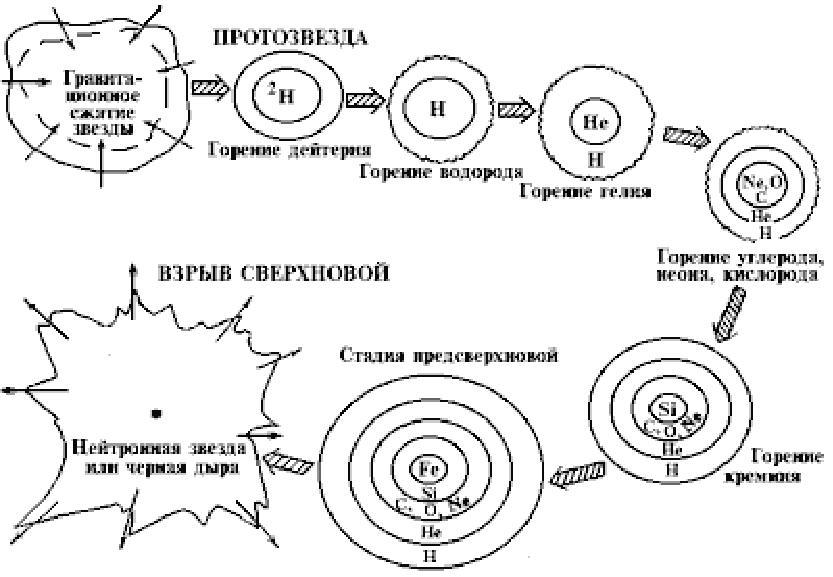
\includegraphics[width=.8\textwidth]{figures/25M-evo-steps.gif.pdf}

	% Как нам всем я полагаю известно, нуклеосинтез в звездах проходит 
	% в несколько стадий, результатом которых оказывается довольно 
	% разнообразная слоистая структура, особенно в случае тяжелых звезд.
}% }}}

\frame{% White Dwarfs Formation {{{
	\frametitle{Образование белых карликов}
	\centering
	% Pictures {{{
	\begin{columns}
		\column{.5\linewidth}{\begin{center}
			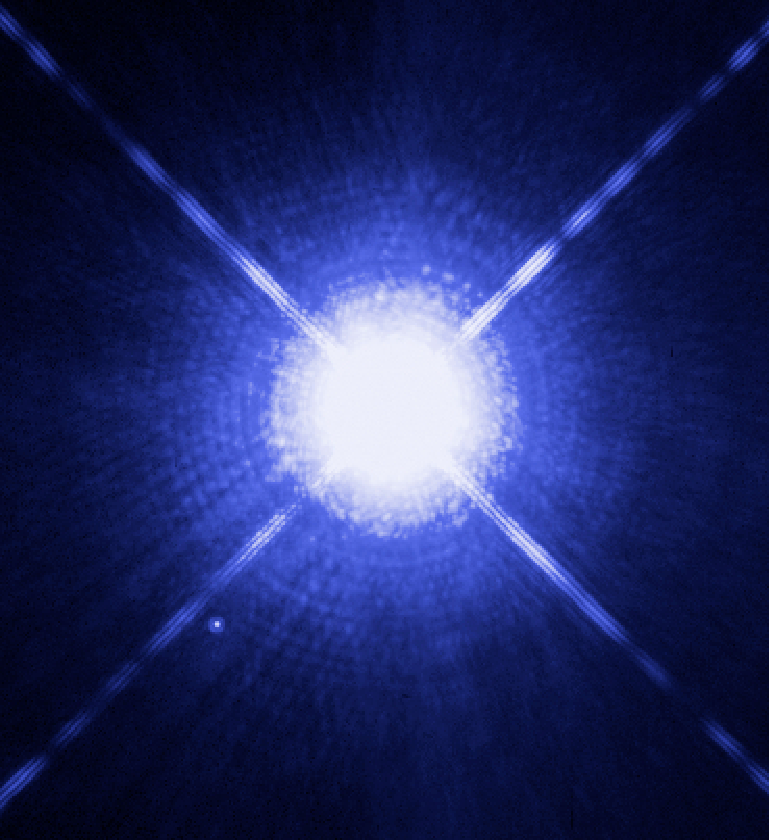
\includegraphics[width=\textwidth]{figures/Sirius_A_and_B_Hubble_photo.jpg.pdf}
			\\
			Сириус А и Б, снимок Хаббл.
		\end{center}}
		\hfill
		\column{.5\linewidth}{\begin{center}
			\vskip-\baselineskip
			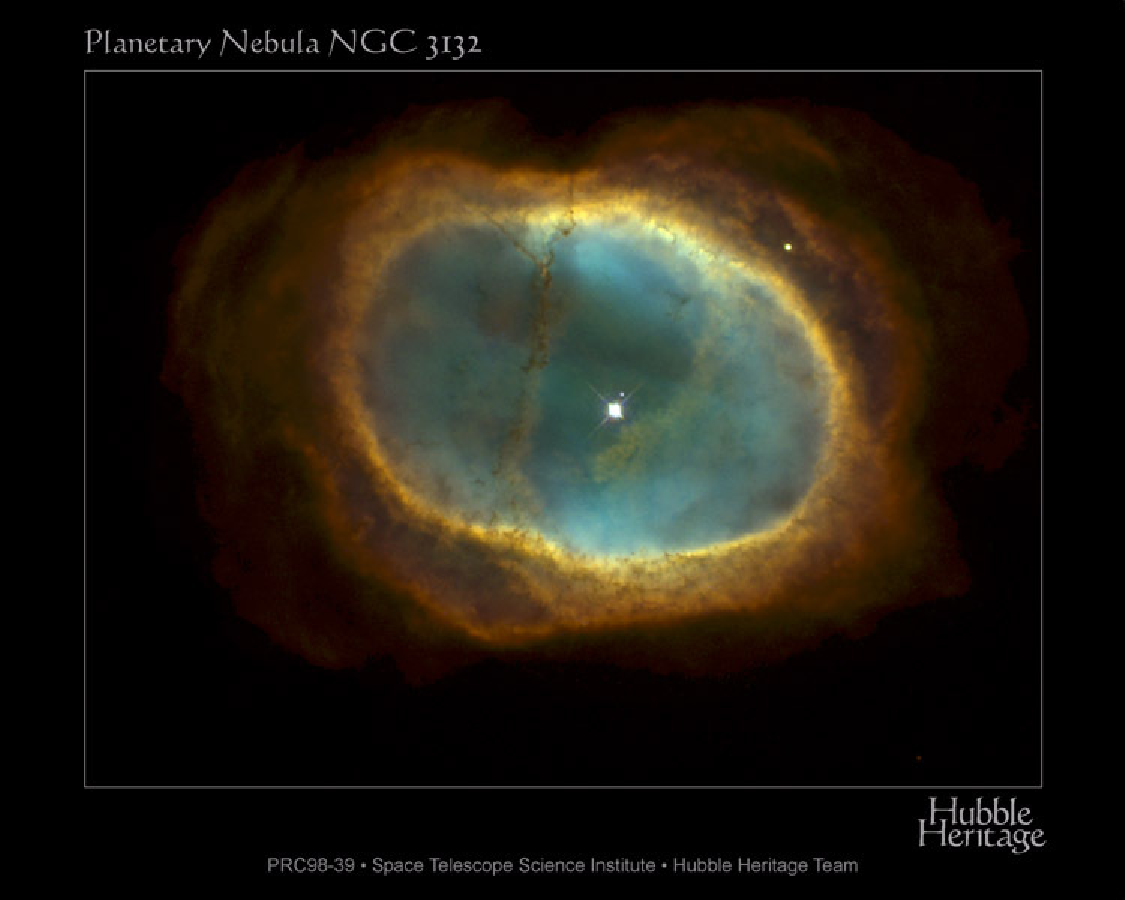
\includegraphics[width=.75\linewidth]{figures/Planetary.Nebula.NGC3132.jpg.pdf}
			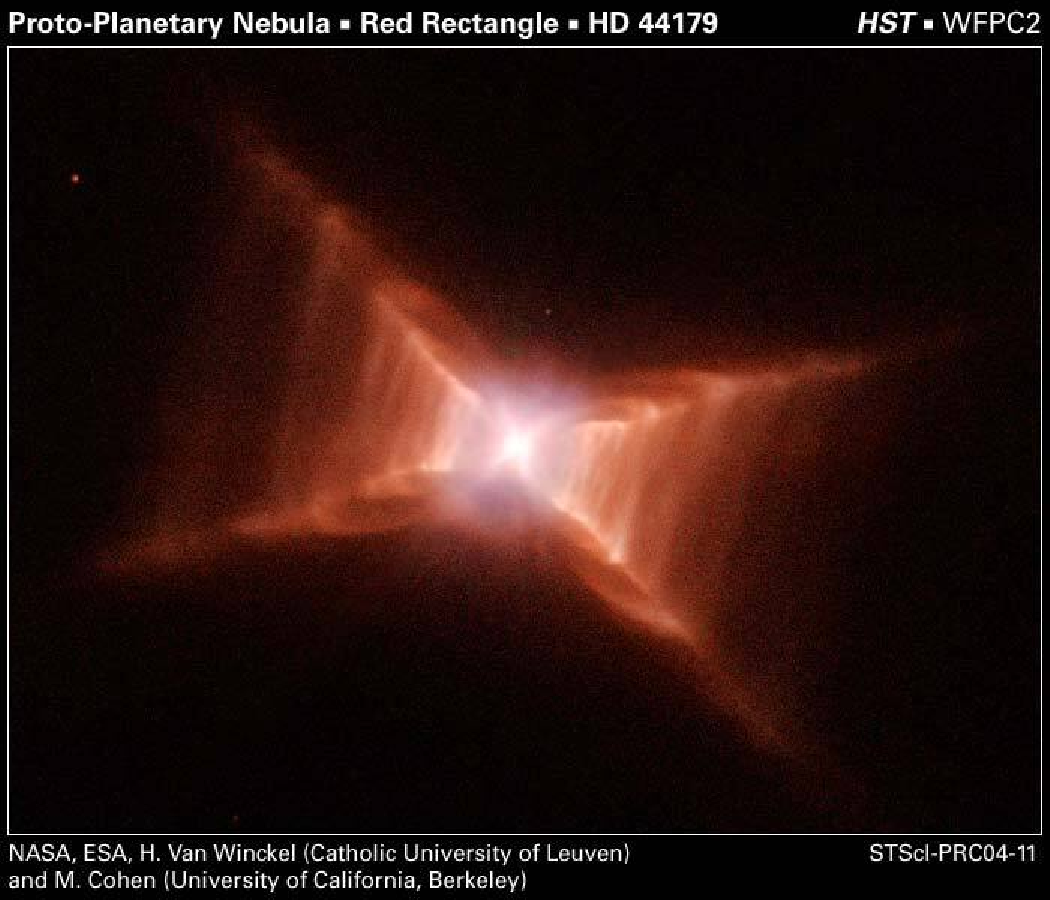
\includegraphics[width=.75\linewidth]{figures/Proto-Planetary.Nebula.HD44179.large.jpg.pdf}
		\end{center}}
	\end{columns}
	% }}}

	% Белые карлики являются конечной стадией эволюции звезд малых 
	% и промежуточных масс. При завершении каждого этапа эволюции 
	% происходит сжатие центра звезды под действием гравитации, и если 
	% общая масса звезды оказывается недостаточно большой, следующий шаг 
	% нуклеосинтеза не запускается. Реакции в центре прекращаются, 
	% а остаются лишь на периферии. А звезда увеличивается в радиусе 
	% и выбрасывает в космос часть своей массы. Этот процесс сравнительно 
	% медленный, но завершается резким срывом всей оставшейся оболочки. 
	% В результате остается только ядро звезды, состоящее из углерода 
	% и кислорода или кислорода, неона и магния. Остатки оболочки, 
	% разнесенные по пространству вокруг белого карлика, называют 
	% планетарной туманностью.
	%
	% Также возможен случай гелиевых белых карликов. В одиночку они могут 
	% образоваться путем выгорания всего или почти всего водорода 
	% в звезде, но это происходит дольше времени жизни вселенной. 
	% Считается, что гелиевые белые карлики могут образовываться 
	% в двухзвездных системах при потере легкой звездой ее водородной 
	% оболочки.
	%
	% Механизм быстрого сброса до сих пор не остается полностью 
	% описанным. Известно, что возможны существенно асимметричные 
	% туманности, как вот тут внизу. На картинке во-первых наблюдаются 
	% волны выбросов, а во-вторых видна сама асимметрия. Это может быть 
	% обусловлено колебаниями оболочки в случае вытянутых звезд.
	%
	% МОЖНО ЕЩЕ РАССКАЗАТЬ ПРО ЭТОТ БРЕД ПРО ТЕМПЕРАТУРУ И НЕСТАБИЛЬНОСТЬ 
	% ТРОЙНОГО АЛЬФА-ПРОЦЕССА
}% }}}

\frame{% Supernova type Ia {{{
	\frametitle{C-O-белый карлик. Сверхновая типа~Ia}
	\centering
	
	\parbox[c]{.48\textwidth}{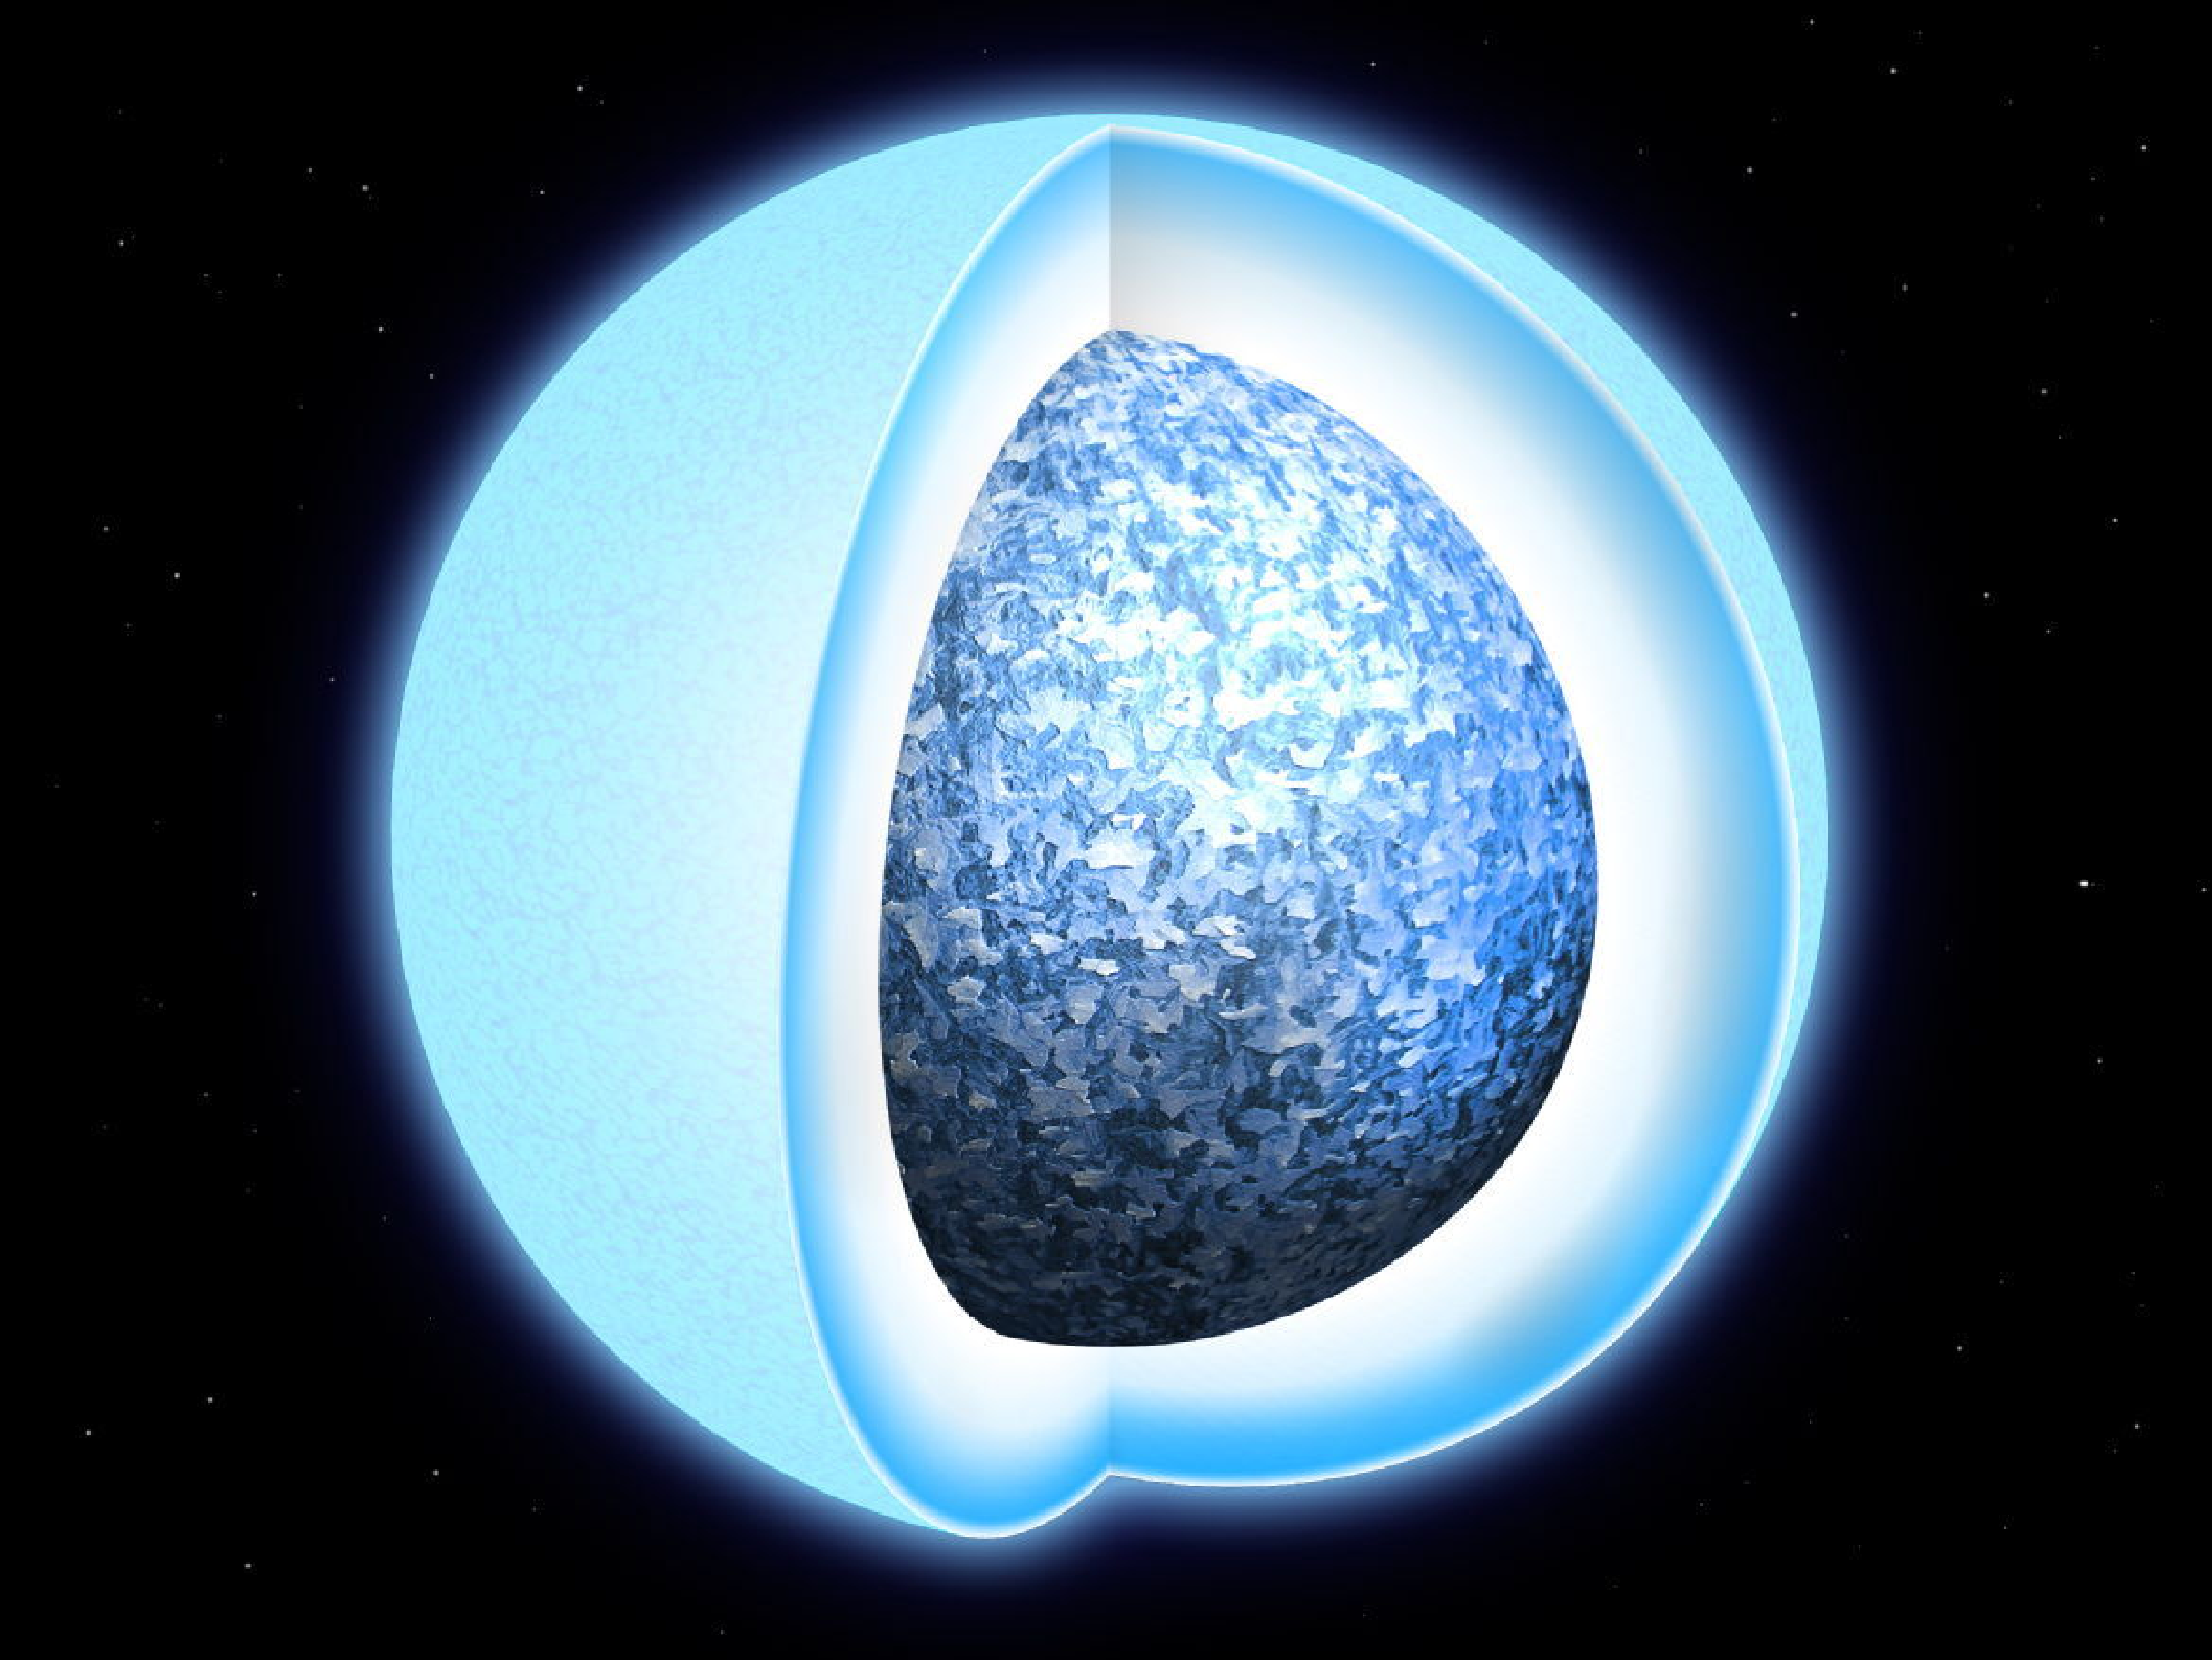
\includegraphics[width=.48\textwidth]{figures/white_dwarf_interior.jpg.pdf}}
	\pause
	\parbox[c]{.48\textwidth}{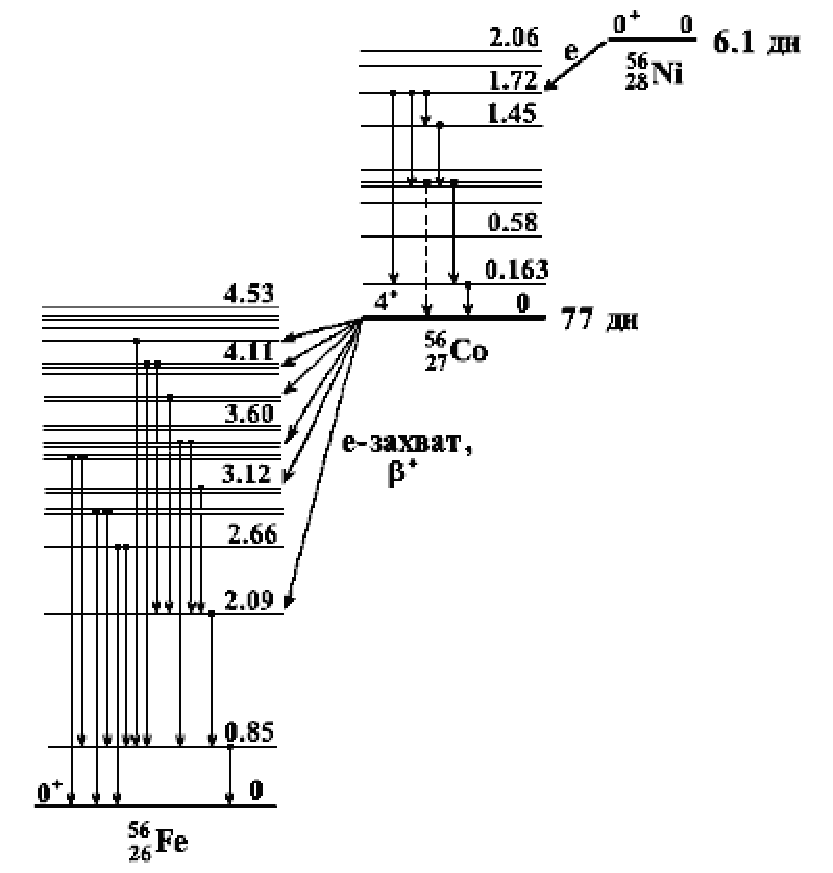
\includegraphics[width=.48\textwidth]{figures/nsf33.gif.pdf}}

	% Чаще всего встречаются углерод-кислородные белые карлики, 
	% поэтому я расскажу про этот случай. Если белый карлик входит 
	% в состав двухзвездной системы, он притягивает вещество со своего 
	% соседа благодаря массе и постепенно наращивает вещество, которое 
	% выступает по сути в роли атмосферы.
	% 
	% При нарастании массы предел коллапса в нейтронную звезду, как мы 
	% находили на семинаре, не достигается. Вместо этого чуть меньшая 
	% масса поджигает реакцию слияния углерода внутри звезды, причем, 
	% в отличие от обычных условий в более тяжелой звезде, давление на 
	% стенки, обусловленное вырожденным электронным газом, не расширяет 
	% их, и происходит очень быстрое выгорание углерода, а затем 
	% и кислорода за секунды. Благодаря таким условиям происходит прямое 
	% слияние кремния, приводящее к образованию ядер железного максимума, 
	% но в особенности большого количества радиоактивного изотопа 
	% никель-56. Он затем распадается с периодом 6 дней в возбужденное 
	% состояние кобальта. Кобальт испускает каскады гамма-квантов 
	% и превращается в железо за период полураспада 77 дней. Железо 
	% образуется во многих возбужденных состояниях, которые затем снова 
	% испытывают каскадные распады. Линии кобальта довольно успешно 
	% наблюдаются в спектрах.
	%
	% В результате взрыва от звезды не остается ничего. Она вся 
	% разлетается в космосе.
}% }}}

\frame{% Supernova type Ia and II {{{
	\frametitle{Светимость взрывов сверхновых}
	\centering
	
	{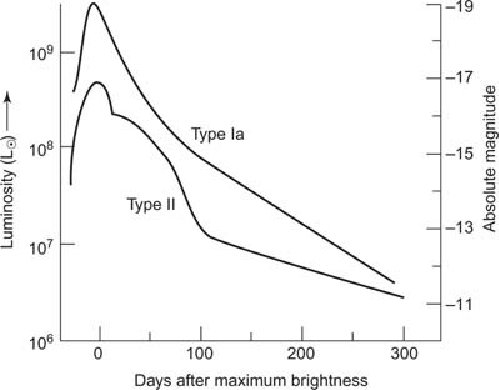
\includegraphics[width=.7\textwidth]{figures/23429.jpg.pdf}}

	% Для наблюдателя основным отличием между взрывами сверхновых будет 
	% форма временной зависимости светимости (на самом деле линии 
	% в спектре, но я временно закрою на это глаза). Как вы знаете, взрывы 
	% сверхновой типа Ia предоставляют довольно полезную возможность 
	% измерять расстояния во вселенной, потому что не зависят от того, при 
	% каких условиях произошли (в пике светимости). Единственной проблемой 
	% оказывается возможность таких взрывов появляться в случае 
	% столкновения белых карликов. В этих условиях возникает кривая 
	% светимости чуть меньшей амплитуды. Однако вероятность таких событий 
	% существенна только в самых старых эллиптических галактиках.
	%
	% Кроме типа 1а существуют типы 1б и ц, и тип 2 тоже подразделяется на 
	% несколько. Тип 1а единственный обусловлен белыми карликами, все 
	% остальные -- коллапсы. Типы 1абц попали под цифру 1 потому что у них 
	% нет линии водорода. Тип 1б это массивная звезда без водородной 
	% оболочки, а ц-- и без водородной и без гелиевой. Образовываться 
	% такое может из-за особой какой-нибудь звездного ветра или из-за 
	% соседа. На этом классификацию трогать я бы перестал.
	%
	% Взрыв сверхновой SN 1987A относят к типу II, но ему были присущи 
	% некоторые черты типа Ia в связи с наличием тех же изотопов никеля. 
	% Схожие черты это наличие линий кобальта и возрастание светимости 
	% в первые дни, обусловленное расширением оболочки и увеличением ее 
	% прозрачности для гамма-квантов, вылетающих из кобальта.
}% }}}

\frame{% Supernova type II {{{
	\frametitle{Сверхновая типа~II}
	\centering

	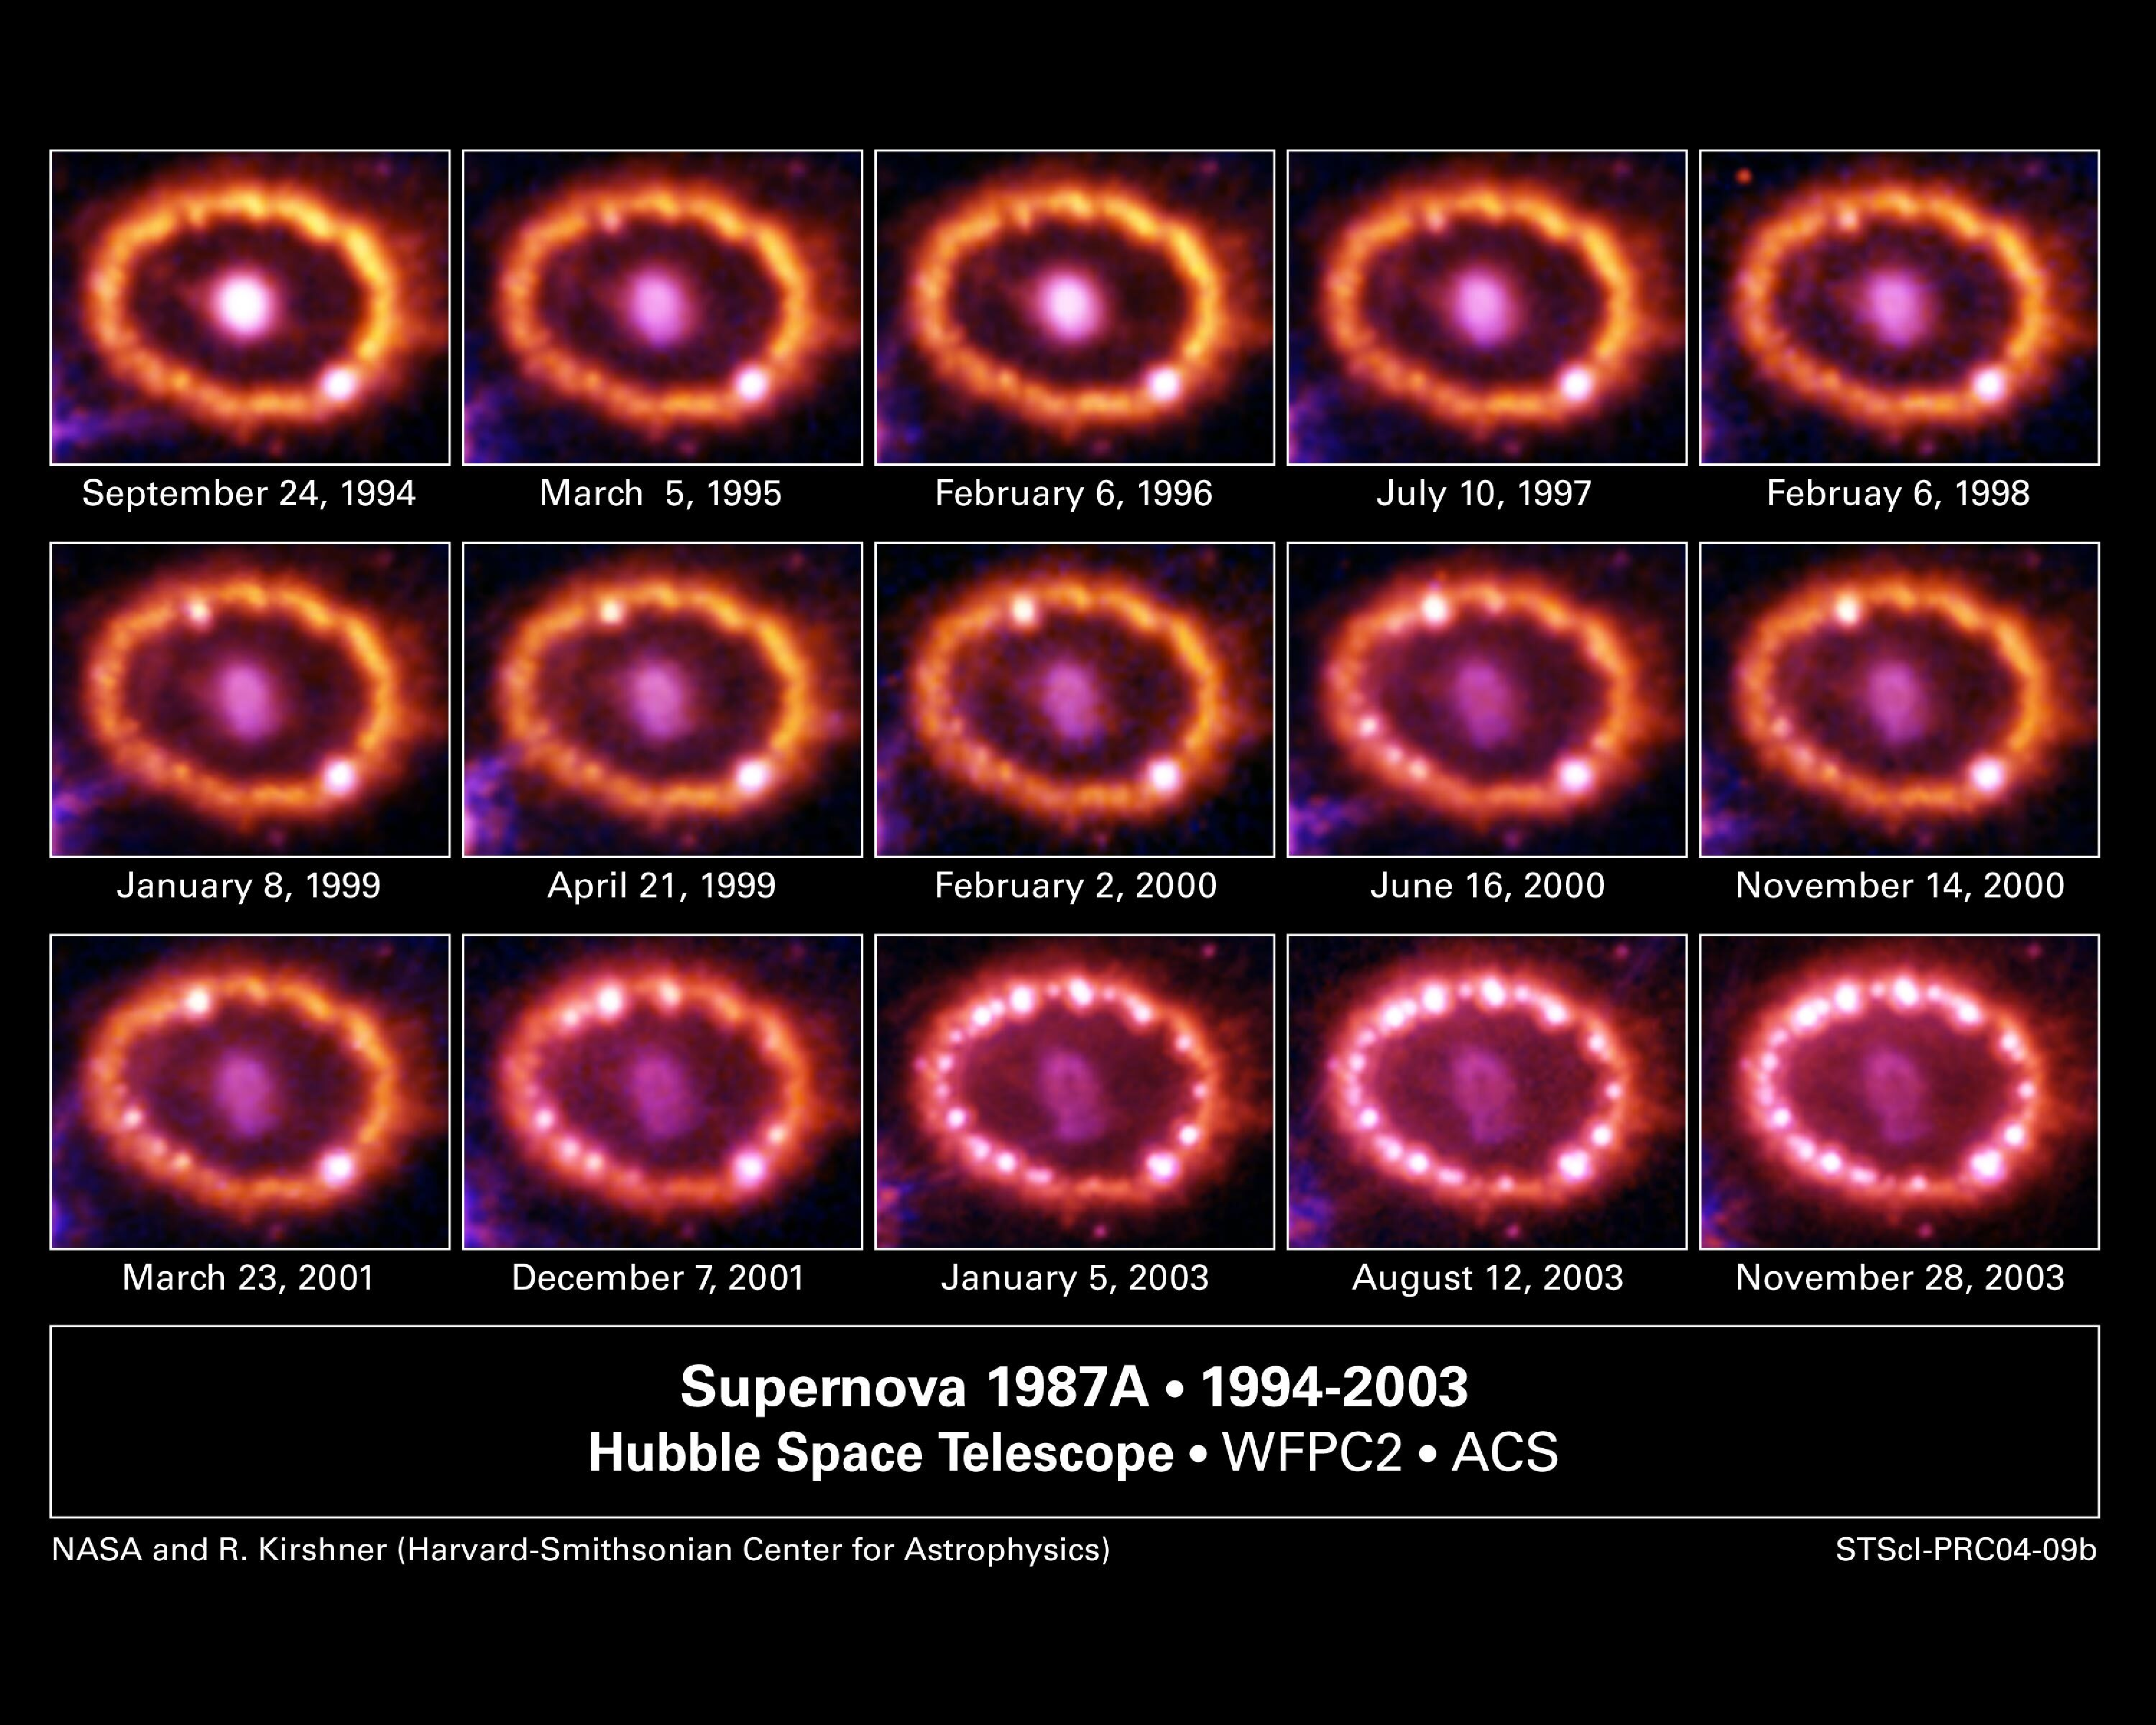
\includegraphics[height=.8\textheight]{figures/print.jpg.pdf}

	% Наиболее тяжелые звезды завершают путь синтеза самостоятельно 
	% и доходят до железного пика в центре звезды. После этого звезда как 
	% обычно сжимается под гравитацией, но теперь возрастание температуры 
	% не приводит к балансировке, поскольку энергия поглощается обратно на 
	% разделение железа и его соседей на легкие ядра, альфа-частицы 
	% и нуклоны. Кроме того большая энергия электронов открывает каналы 
	% е-захвата тоже поглощающие энергию. Вещество оболочки падает 
	% ускоренно на центр, что провоцирует ускорение синтеза в ней. Большее 
	% сжатие приводит к еще более активному е-захвату, и в центре 
	% образуется нейтронная звезда, а нейтрино уносят колоссальную 
	% энергию. Сжатие при этом заканчивается и отраженная ударная волна 
	% срывает всю оболочку. Вместо отраженной волны оболочка могла бы быть 
	% сорвана нейтрино, для этого понадобился бы только один процент их 
	% энергии. При срыве оболочки в ближнем к центру слое температура 
	% поднимается до пугающих значений и запускает взрывной нуклеосинтез. 
	% На данный момент нельзя с точностью сказать, какие именно элементы 
	% оказываются в космосе, образованные в медленных процессах при 
	% эволюции звезды или образованные за короткое время самого взрыва.
	%
	% Сверхновая SN 1987A снова поддерживает нашу модель тем, что вместе 
	% с фотонами тогда были зарегистрированы нейтрино.
}% }}}

\frame{% Supernova type II -- Black Hole {{{
	\frametitle{Сверхновая типа~II. Черная дыра}
	\centering

	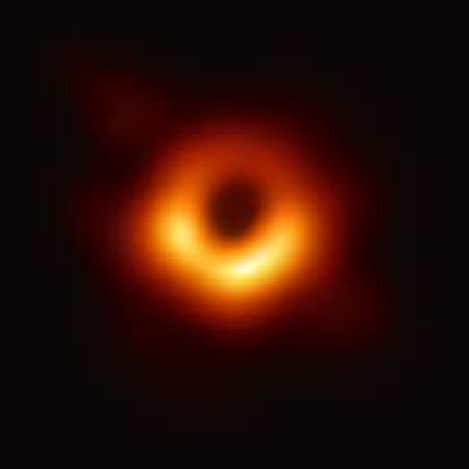
\includegraphics[height=.8\textheight]{figures/download.jpeg.pdf}
	
	% Для звезд еще тяжелее прежних давление вырожденного газа нейтронов 
	% не в состоянии препятствовать гравитации, нейтронная звезда 
	% сжимается еще сильнее и образует черную дыру. Для этого нужна масса 
	% 3 М. Подобное произойдет, если нейтронная звезда притянет откуда-либо 
	% еще недостающую массу или же столкнется с чем-нибудь еще и окажется 
	% тяжелее того предела.
	%
	% Кроме того, в сверхновых создаются условия благоприятные, насколько 
	% это слово вообще здесь можно применить, благоприятные для r- 
	% и rp-процессов.
}% }}}

\frame{% Conclusions {{{
	\frametitle{Выводы}

	\null\vfill\null
	Взрывы сверхновых
	\begin{itemize}
		\item являются важным механизмом выброса продуктов звездного 
			нуклеосинтеза в космос, 
		\item обуславливают создание нейтронных звезд и черных дыр, 
		\item могут предоставлять необходимые для r- и rp-процессов условия, 
		\item позволяют проверять более сложные модели поведения ядер 
			в экстремальных условиях,
			% любая проверка нашего понимания это всегда хорошо 
		\item позволяют определять расстояния между галактиками (тип Ia).
	\end{itemize} 
	% Кроме того мы в первый раз или в очередной раз узнали о современных 
	% представлениях касательно механизмов самих взрывов сверхновых.
	
	\pause

	\null\vfill\null
	\begin{center}
		Спасибо за внимание!
	\end{center}
	\null\vfill\null
}% }}}

\end{document}
